\chapter{MISCELLANEOUS}

\section{Machine Constant Check (MACHINE CONSTANT MENU)}

Machine-specific data is stored in the machine constant memory \textbf{CM} of the control system.

These values are recorded in the machine constant list within this memory and can be checked at any time.

The check must be performed using the machine constant list located inside the machine's electrical cabinet.

\procedure

\begin{itemize}
    \iconitem{Press the \textbf{MANUAL} key.}{manual.jpg}
\end{itemize}

\vspace{.5cm}

\begin{itemize}
    \iconitem{Press the \textbf{CONST. MEM} key.}{const_mem.jpg}
\end{itemize}

The machine constants table appears on the screen:

\begin{center}
    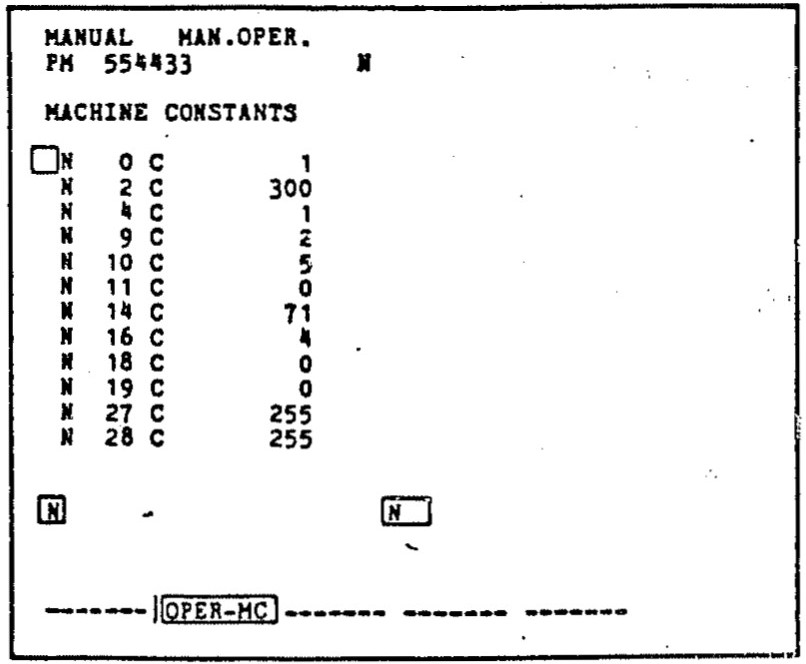
\includegraphics[width=0.6\linewidth]{machine_constants.jpg}
\end{center}

\begin{itemize}
    \iconitem{Move the cursor to the machine constant number \textbf{N} to be checked using the up/down command keys.}{up.jpg, down.jpg}
\end{itemize}

If one of the up/down command keys is held down for more than one second, the cursor automatically jumps from one machine constant number \textbf{N} to the next.

If the required machine constant is outside the displayed portion of the list, it may be more efficient to follow the search procedure described below.

\newpage

\begin{itemize}
    \item Enter the machine constant number \textbf{N} on the numeric keypad.
    \iconitem{Press the \textbf{ENTER} key.}{enter.jpg}
\end{itemize}

\vspace{.5cm}

\begin{itemize}
    \iconitem{Press the \textbf{SEARCH} key to start the search procedure.}{search.jpg}
\end{itemize}

After pressing the key, the cursor is positioned in front of the machine constant number \textbf{N} being searched.

The lower cursor on the screen is now positioned at address letter \textbf{C}.  
It must be returned to address letter \textbf{N} if the search is to continue according to the described procedure.

After completing the machine constant check:

\begin{itemize}
    \iconitem{Press the \textbf{MANUAL} key.}{manual.jpg}
\end{itemize}
\vspace{.5cm}
\section{Software Number Check}

The control system in its supplied state is clearly identified by the software number.

This number must always be indicated when requesting information.

The software number is stored in the machine constant memory \textbf{CM} and can be displayed on the visualization screen at any time.

\procedure

\begin{itemize}
    \iconitem{Select \textbf{MANUAL} and \textbf{MENU} to access DIAGNOSTIC (7).}{manual.jpg, menu.jpg}
\end{itemize}

\begin{itemize}
    \item Select \textbf{CONFIGURATION CHECK} (1).
\end{itemize}

The software number is displayed on line 9.

Once the software number check is complete:

\begin{itemize}
    \iconitem{Press the \textbf{MANUAL} key.}{manual.jpg}
\end{itemize}

\newpage

\section{Display of Signal States at System Input and Output Points}

Using the function key \textbf{F5 (IN-OUT)}, it is possible to display the signal states \textbf{0} and \textbf{1} of the system's \textbf{IN} inputs and \textbf{OUT} outputs. This can be done even before the start of a program or during its execution to allow for diagnostic procedures.

The signal states can be continuously monitored during startup and while the program is running. They are displayed in \textbf{TEACH IN}, \textbf{SINGLE}, and \textbf{AUTO} operating modes.

\procedure

\begin{itemize}
    \iconitem{Press the \textbf{MANUAL} key.}{manual.jpg}
\end{itemize}

\vspace{.5cm}

\begin{itemize}
    \iconitem{Press the \textbf{TEACH IN}, \textbf{AUTO}, or \textbf{SINGLE} button.}{teach_in.jpg, auto.jpg, single.jpg}
\end{itemize}

\vspace{.5cm}

\begin{itemize}
    \iconitem{Press the function key \textbf{F5 (IN-OUT)}.}{f5.jpg}
\end{itemize}

A table displaying the input and output signal states of the control system appears on the screen:

\begin{center}
    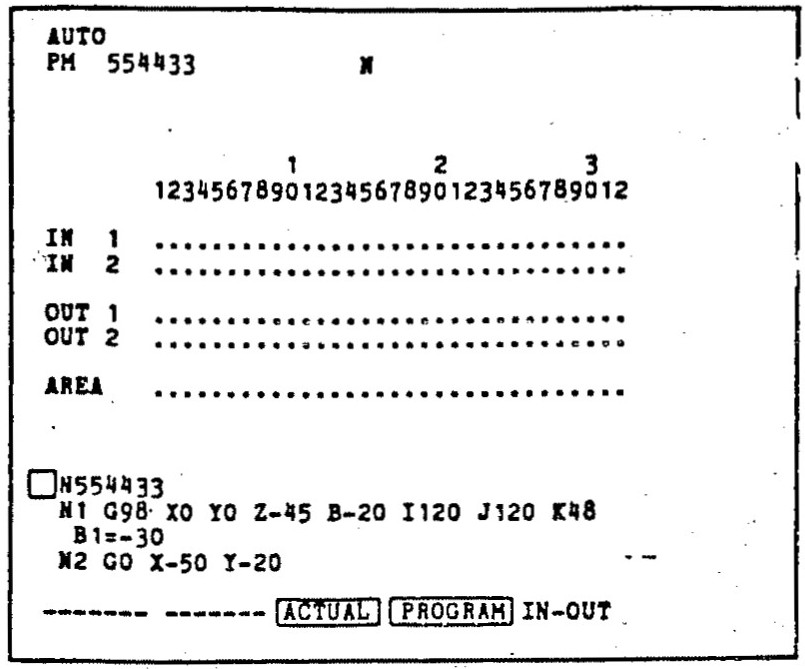
\includegraphics[width=0.6\linewidth]{signal_states_table.jpg}
\end{center}

After pressing the \textbf{START} button, both the program and the signal states can be monitored simultaneously on the screen.

The \textbf{IN-OUT} mode can be canceled at any time while the program is running.

\begin{itemize}
    \iconitem{Press the function key \textbf{F3 (ACTUAL)}.}{f3.jpg}
\end{itemize}

Pressing the key makes the normal program execution reappear on the screen in \textbf{TEACH IN}, \textbf{SINGLE}, or \textbf{AUTO} modes.

During program execution the system's input and output states can be canceled at any time using the function key \textbf{F3 (ACTUAL)}.

\newpage

\setcounter{section}{4}
\section{Modification of Machine Constants}

Machine-specific data is stored in the machine constant memory \textbf{CM}.

These values have been stored by the machine manufacturer and, as a rule, should not be modified.

Without special authorization from the machine manufacturer, only the machine constants listed in a separate machine constant list may be modified.

\procedure

\begin{itemize}
    \iconitem{Press the \textbf{MANUAL} key.}{manual.jpg}
\end{itemize}

\vspace{.5cm}

\begin{itemize}
    \iconitem{Press the \textbf{CONST. MEM} key.}{const_mem.jpg}
\end{itemize}

\vspace{.5cm}

\begin{itemize}
    \iconitem{Press the function key \textbf{F2 (OPER-MC)}.}{f2.jpg}
\end{itemize}

The screen now displays only the machine constants that can be modified without needing to switch the lockout switch located in the machine’s electrical cabinet.

All other constant values \textbf{C} may only be modified with explicit authorization from the machine manufacturer.

\procedure

\begin{itemize}
    \iconitem{Press the \textbf{MANUAL} key.}{manual.jpg}
\end{itemize}

\vspace{.5cm}

Set the lockout switch used for unlocking and locking the machine constant memory to position \textbf{1}.

\marginnoteicon[2cm]{14.5cm}{lockout_switch_on.jpg}

This switch is located in the machine's electrical cabinet.

The machine constant list appears on the screen:

\begin{center}
    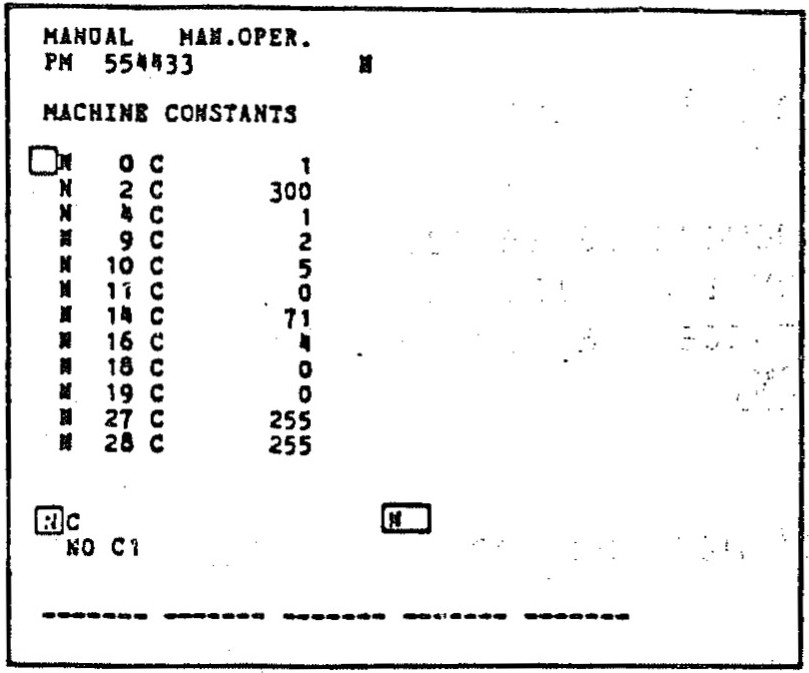
\includegraphics[width=0.6\linewidth]{machine_constants_list.jpg}
\end{center}

\textbf{"NO C1"} is displayed on line 21 of the screen.

\begin{itemize}
    \iconitem{Move the cursor to the machine constant number \textbf{N} to be modified using the up/down command keys.}{up.jpg, down.jpg}
\end{itemize}

\newpage

If the machine constant to be modified is outside the displayed portion of the list, it is more efficient to perform a search following the procedure described below.

\begin{itemize}
    \item Enter the machine constant number \textbf{N} on the numeric keypad.
    \iconitem{Press the \textbf{ENTER} key.}{enter.jpg}
\end{itemize}

\vspace{.5cm}

\begin{itemize}
    \iconitem{Press the \textbf{SEARCH} key to start the search procedure.}{search.jpg}
\end{itemize}

Pressing the key places the cursor in front of the machine constant number \textbf{N} found.

The lower cursor on the screen is now positioned at address letter \textbf{C}.

\begin{itemize}
    \item Enter the machine constant value \textbf{C} on the numeric keypad (without a decimal point).
    \iconitem{Press the \textbf{ENTER} key.}{enter.jpg}
\end{itemize}

Pressing the key makes the entered machine constant value \textbf{C} appear on line 14 of the screen, allowing it to be verified again.

\begin{itemize}
    \iconitem{Press the \textbf{STORE} key.}{store.jpg}
\end{itemize}

Pressing the \textbf{STORE} key saves the new value \textbf{C} of the selected machine constant for number \textbf{N} in the machine constant memory \textbf{CM}.

At the end of the data entry procedure for machine constants:

\begin{itemize}
    \item Set the lockout switch used for unlocking and locking the machine constant memory from position \textbf{1} (unlock) back to position \textbf{0} (lock).
\end{itemize}

This switch is located in the machine's electrical cabinet.

\marginnoteicon[2cm]{13cm}{lockout_switch_off.jpg}

For safety reasons, the machine's hydraulic and electrical systems are disabled during the locking of the machine constant memory.

\begin{itemize}
    \iconitem{Restart the machine's hydraulic and electrical systems (see paragraph 1.1).}{hydraulic_on.jpg}
\end{itemize}

The signal \textbf{REF.-POINT} displayed on line 1 of the screen indicates that the machine axis reference points must be engaged (see paragraph 1.2).

\newpage

\subsection{Introduction and Retrieval of Machine Constants}

The machine manufacturer has provided a perforated tape containing the machine-specific data recorded in the machine constant memory \textbf{CM} of the control system.

This \textbf{perforated tape with machine constants}, along with a printed list of machine constants, is stored in the machine’s electrical cabinet.

In very rare cases, such as after the machine has been out of service for several weeks, it is necessary to re-enter the machine constants stored on this perforated tape back into the machine constant memory.

\procedure

Before data entry, the \textbf{C} values of the machine constants must be manually entered into the machine constant memory for the machine constant numbers \textbf{N726} and \textbf{N727}.

The values \textbf{C} can be taken from the printed machine constant list.

Manual entry must follow the procedure described in paragraph 10.5.

After manual entry:

\begin{itemize}
    \iconitem{Press the \textbf{DATA IN/OUT} key.}{data_in_out.jpg}
\end{itemize}

\vspace{.5cm}

\begin{itemize}
    \iconitem{Press the function key \textbf{F1 (INPUT)} to start the data entry procedure.}{f1.jpg}
\end{itemize}
\vspace{1cm}
At the end of the entry procedure:

\begin{itemize}
    \item Set the lockout switch used for unlocking and locking the machine constant memory from position \textbf{1} (unlock) back to position \textbf{0} (lock).
\end{itemize}

\marginnoteicon[2cm]{14cm}{lockout_switch_off.jpg}

\notes

If a perforated tape reader is unavailable, the machine-specific data must be extracted from the machine constant memory \textbf{CM} and stored on an appropriate external data medium. This ensures that it can be re-entered into the machine constant memory when needed.

Machine constant retrieval can be performed by pressing the keys \textbf{"CONST.MEM."}, \textbf{"DATA IN/OUT"}, and \textbf{F2} sequentially.

\newpage
\setcounter{section}{6}
\section{Functions of Control Elements on the Machine Operation Panel}

\begin{enumerate}
    \item Function keys
    \item Function keys
    \item Function keys
    \item Function keys
    \item Function keys
    \item Selection of the \textbf{main program memory}
    \item Selection of the \textbf{tool data memory}
    \item Machine constant memory
    \item Operating mode: \textbf{input/output of data} from an external information support or to an external information support
    \item Entry of calculation symbols for parameter calculations
    \item Entry of \textbf{numerical values and decimal points}. \\Sign conversion and block identification (maskable blocks \textbf{/N})
    \item Clearing of error signals and input signals on the panel
    \item Entry of the \textbf{equal sign (=)}
    \item Acceptance of data into input memory
    \item Selection of menus on the screen
    \item Data storage
    \item Cursor control \textbf{"left-right"}
    \item Cursor control \textbf{"up-down"}
    \item Program or block search
    \item Rotation of the tool magazine \textbf{left or right} (the first key pressed determines the rotation direction)
    \item \textbf{Clamping and unclamping} of the tool in the working spindle
    \item \textbf{Pump on/off} for coolant activation (when the auxiliary function \textbf{"coolant ON"} is activated)
    \item Axis movement in manual mode
    \item Step movement of the spindle
    \item Adjustment of spindle speed \textbf{+/- 20\%}
    \item Selection of the programmed spindle speed
    \item Keys for incremental movement
    \item Step movement in continuous mode
    \item \textbf{Feed hold (HALT)}
    \item Intervention key affecting feed speeds
    \item Programmed feed
    \item Selection of \textbf{TEACH IN mode} (manual data entry)
    \item Selection of \textbf{SINGLE mode} (execution of the program block by block)
    \item Selection of \textbf{AUTO mode} (automatic program execution)
    \item Selection and cancellation of the \textbf{optional block skip} function
    \item Selection of \textbf{MANUAL mode} (manual operation)
    \item Reset to initial state
    \item Stop of the lead screw and working spindle
    \item \textbf{Feed stop (STOP)}
    \item \textbf{Start (cycle start)}
\end{enumerate}

\newpage

Layout of Control Elements on the Machine Operation Panel

\begin{center}
    \hspace{-3.5cm} % Adjust the value to shift further left
    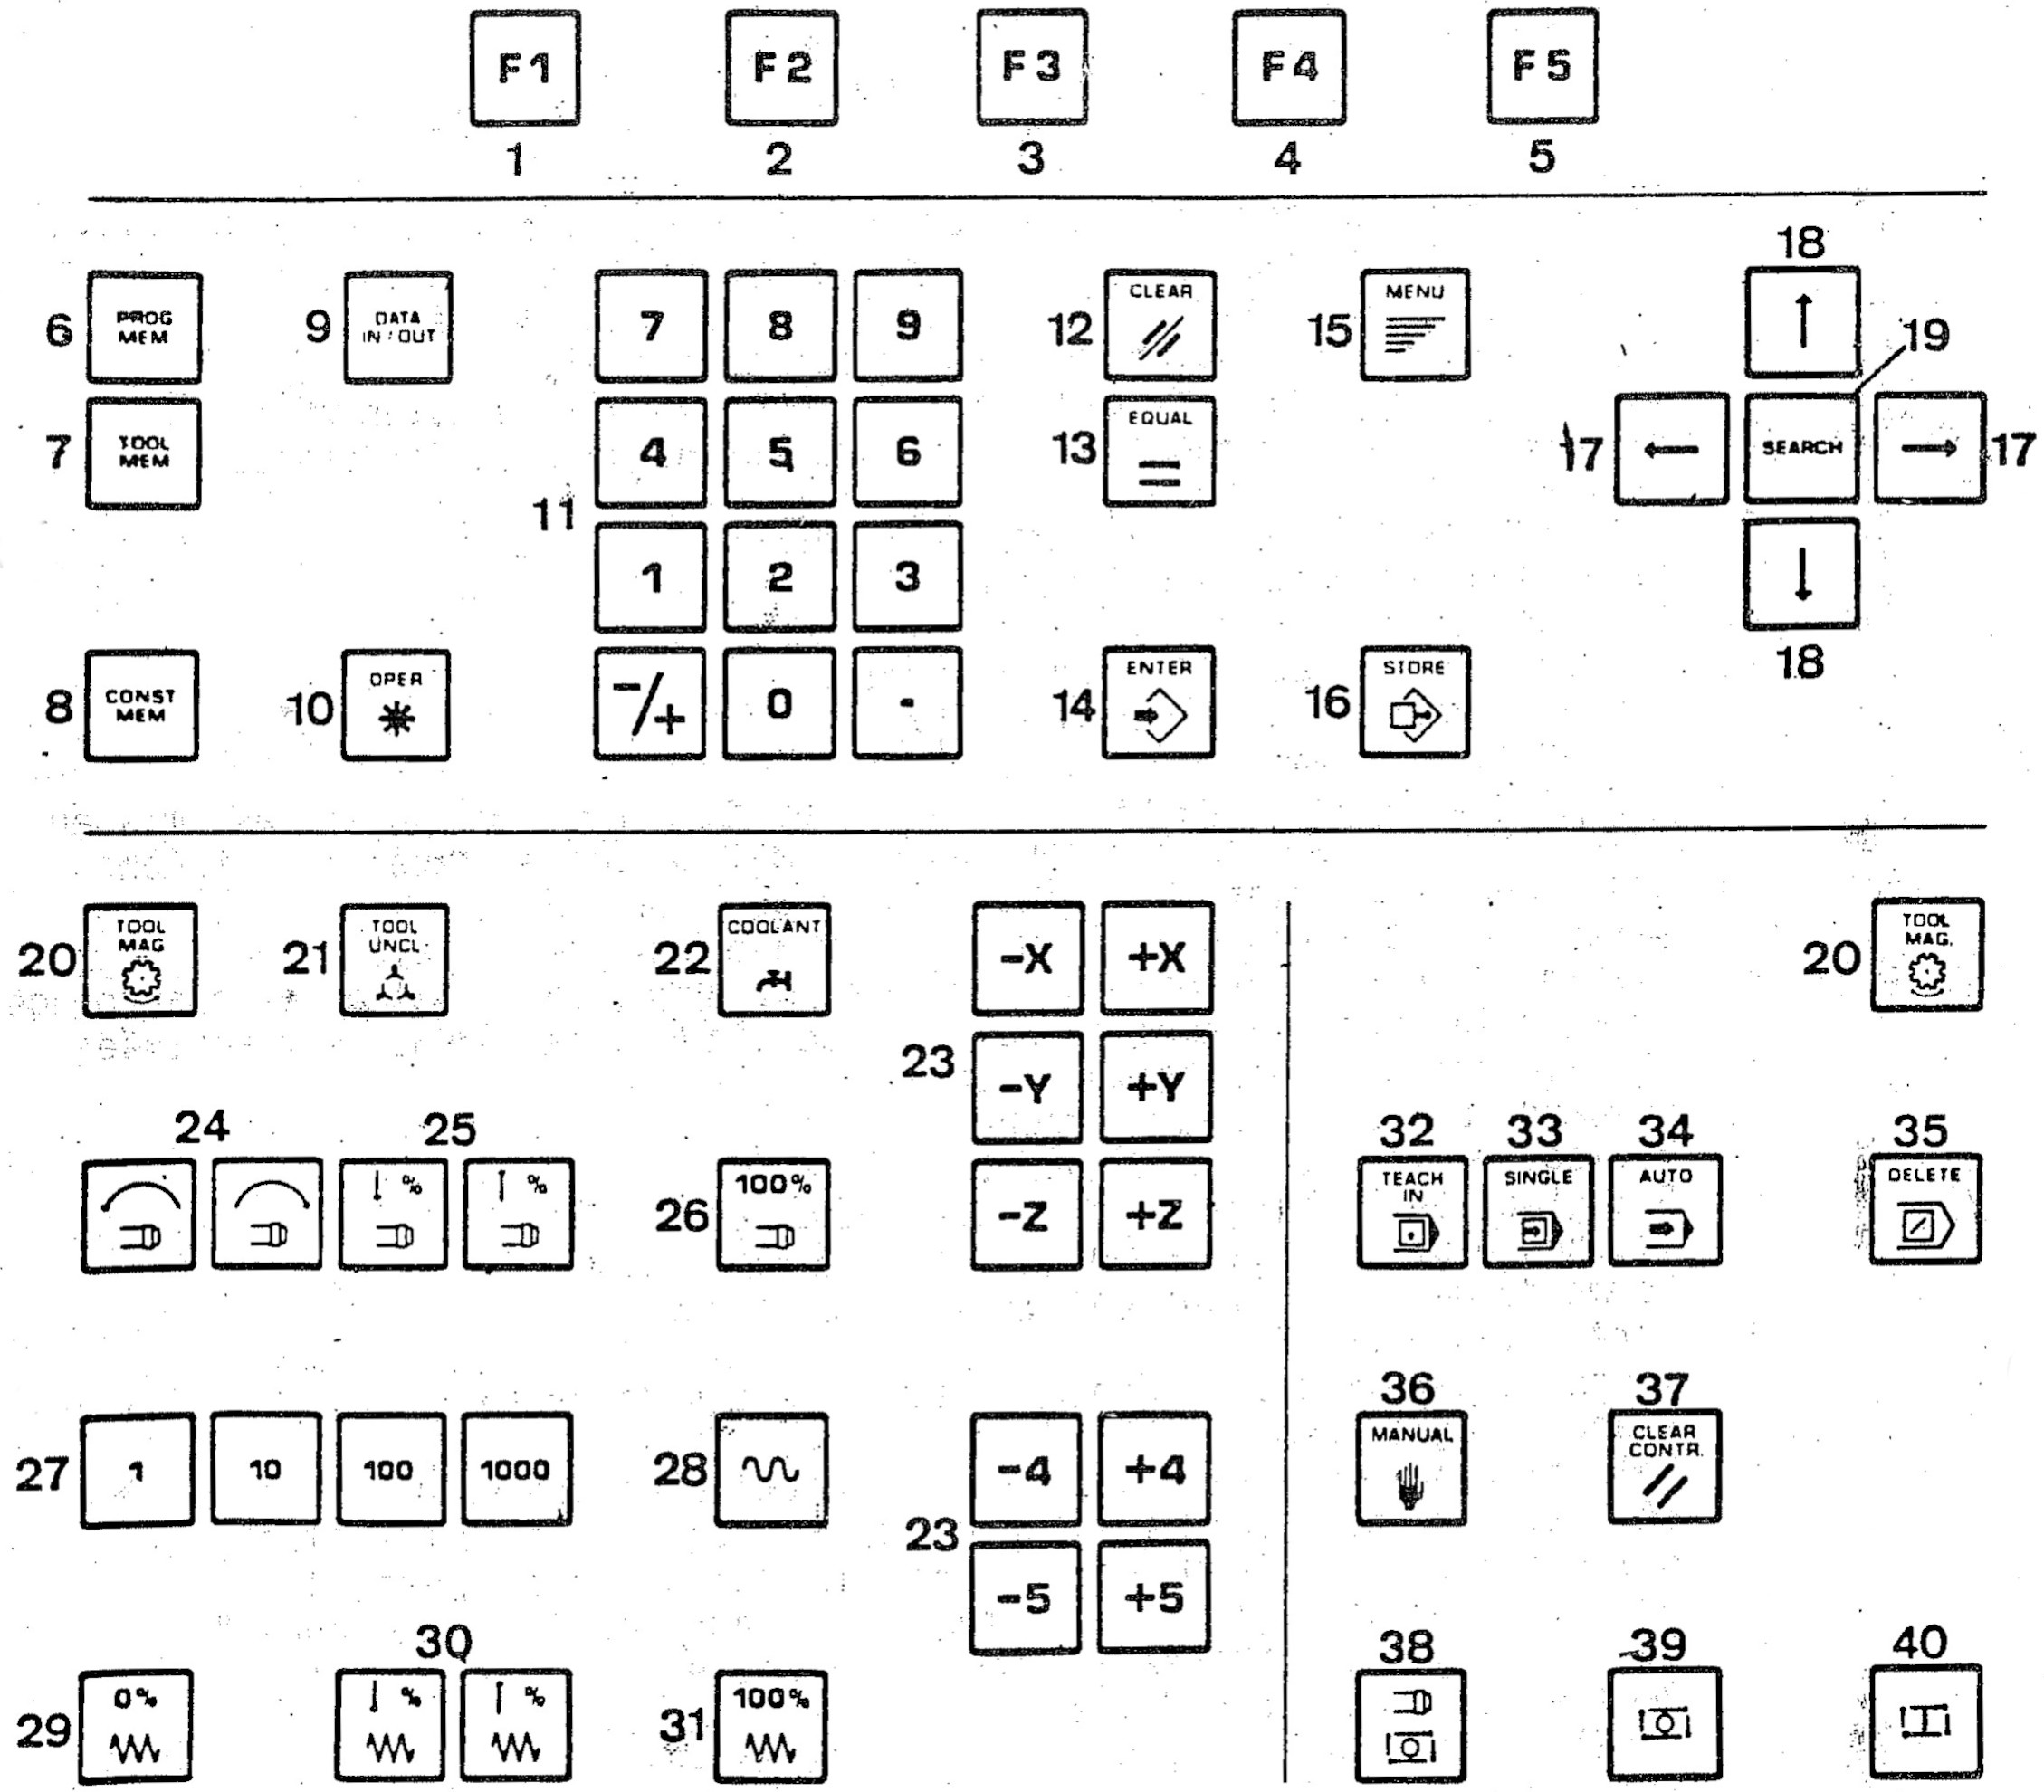
\includegraphics[width=1.2\linewidth]{control_panel_layout.jpg}
\end{center}